\documentclass{article}
\usepackage[screen]{geometry}
\usepackage{alltt,xcolor}
\usepackage[utf8]{inputenc}
\usepackage{listings}
\usepackage{graphicx}
\lstset{escapechar=\@,language=C++,keywordstyle=\color{blue},showstringspaces=false}
\begin{document}
\large 
\section*{Specification}
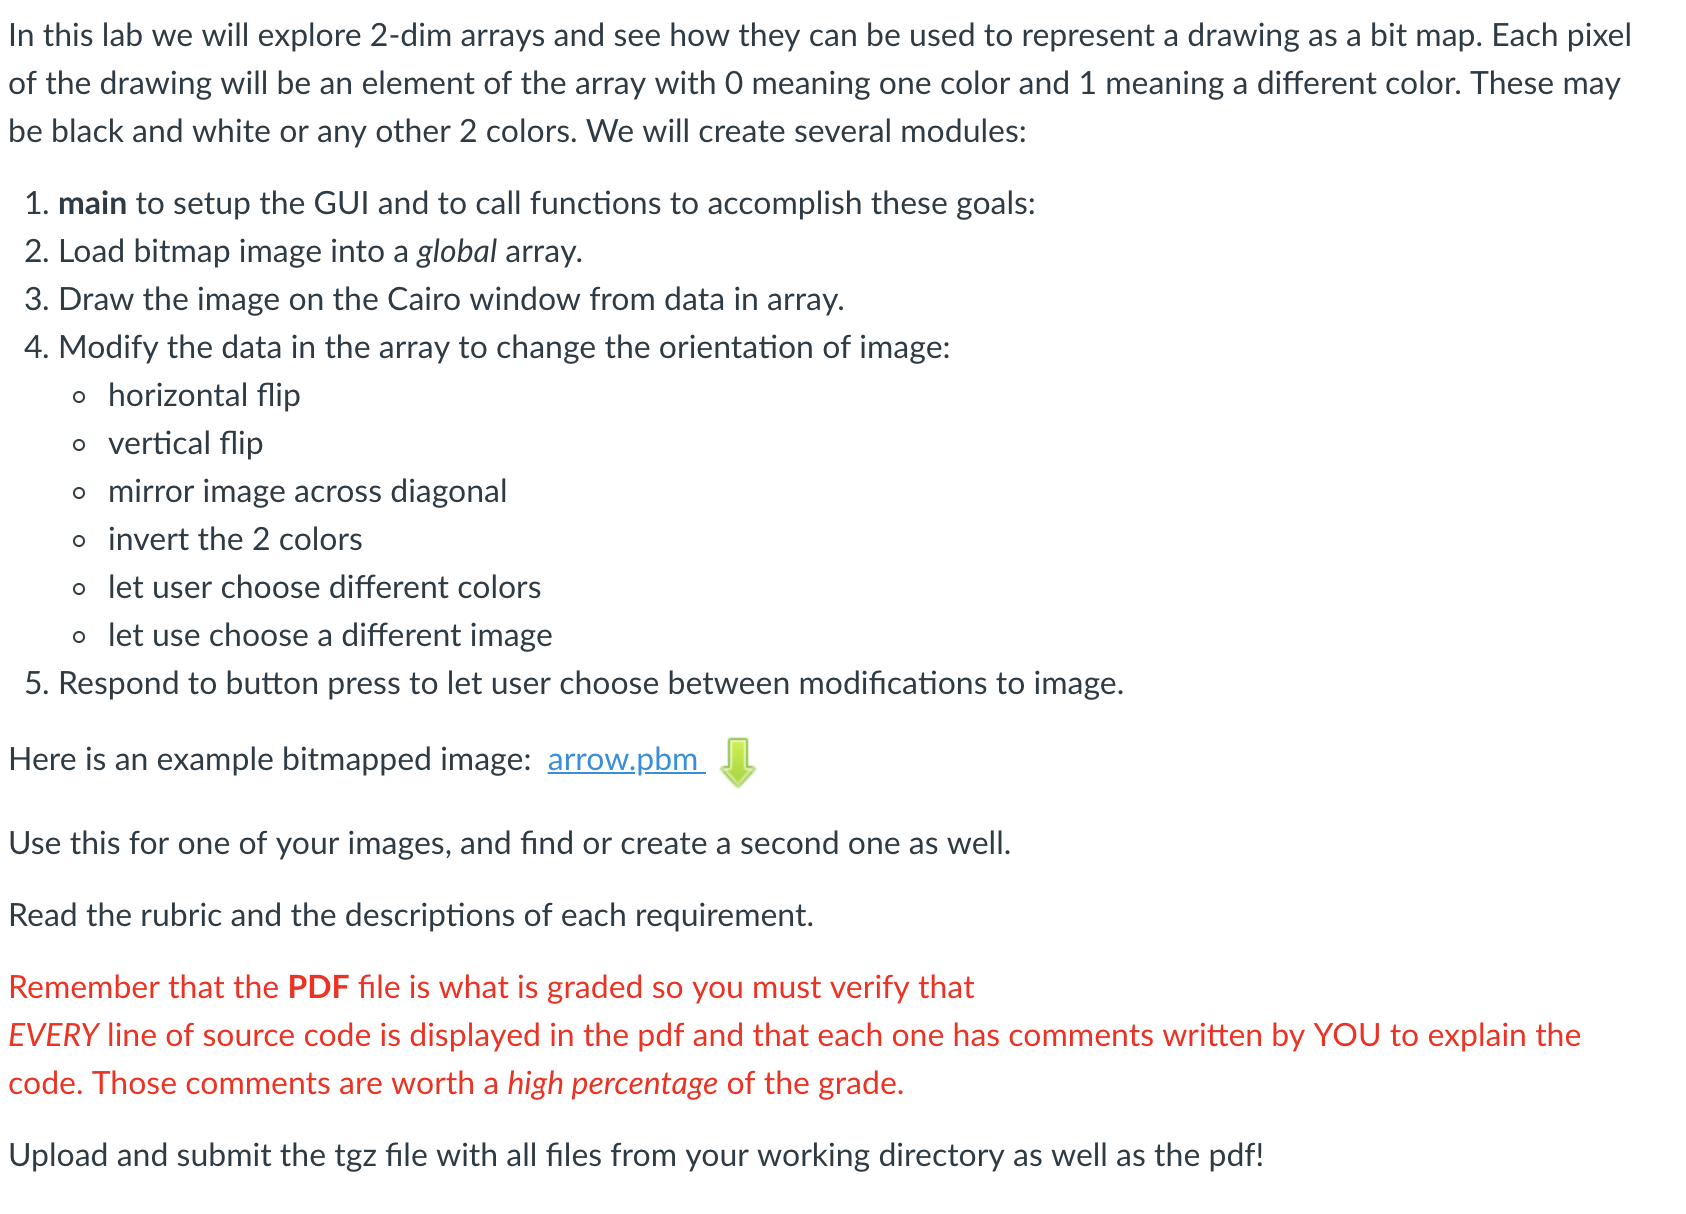
\includegraphics[width = 15cm, height = 11cm]{lab51.png}
\newpage\section*{Analysis}
\begin{description}
	\item[Input] a bit map(one of the two) as a string from our pbm file.(User's choice of 
	colors, way of modify...)
	\item[Preocess] Store the string into the global array, where 0 means one color and 1 means a different color. When the user click the buttons, modify the image by modify (the data which stored in) the global array based on which button the user clicked.(respond to user's input)
	\item[Output] Show a bit map which is modified by our functions and 
	user's choices ,and the program uses our 2-dim array to draw it.
\end{description}
\newpage\section*{Design}
\begin{itemize}
	\item We have a function for flip vertically named flipv, 
	it gets array of integer as input and then the change the 
	position of the bit from (x,y) into (x,-y)in the coordination.
	\item We have a function for flip color of the image named 
	flipc, it gets array of integer as input and then change all 
	the value in it from 1 into 0, all the 0 into 1.
	\item We have a function for flip horizontally named fliph, 
	it gets array of integer as input and then use the change 
	the position of the bit from (x,y) into (-x,y)in the coordination.
	\item We have two function for flip diagonally named flipd1 and 
	flipd2, they get array of integer as input and then swap all the 
	value in it symmetrically along either diagonal.
	\item We have a function named drawCB ,which uses cairo for choose color, 
	add text, make the window....It will help us create the window.
	\newpage
	\item We have a function named goCB, it use fl\_choice() to create 
	buttons and let user do some choices to modify the image :
		\item horizontal flip
		\item vertical flip
		\item mirror image across diagonal
		\item invert the 2 colors
		\item let user choose different colors
		\item resize it by 10 or 15
	\item We have a function for load the image named load\_image, 
	it gets the pbm file as a string and then store the value in 
	the string into the array(which can be shown as a bit map).
	\item We have a main function which calls the fl\_choice to let  
	user choose and load a image, make the window(title,size), and calls 
	functions to create buttons and the functions we created,etc.
\end{itemize}
\newpage\section*{Implementation}
\lstinputlisting{lab.cpp}
\newpage\section*{Test}

\subsection*{Testcase of choosing a differntent image(it runs well)}
\begin{itemize}
	\item When the user execute our program,the user will see our first window like that,which tells the user to select an image.After the user selected, the one the user selected will be loaded into our program and shows in the window.
	\item (In all the testcases below, I only choose one of the two images as a sample)
\end{itemize}
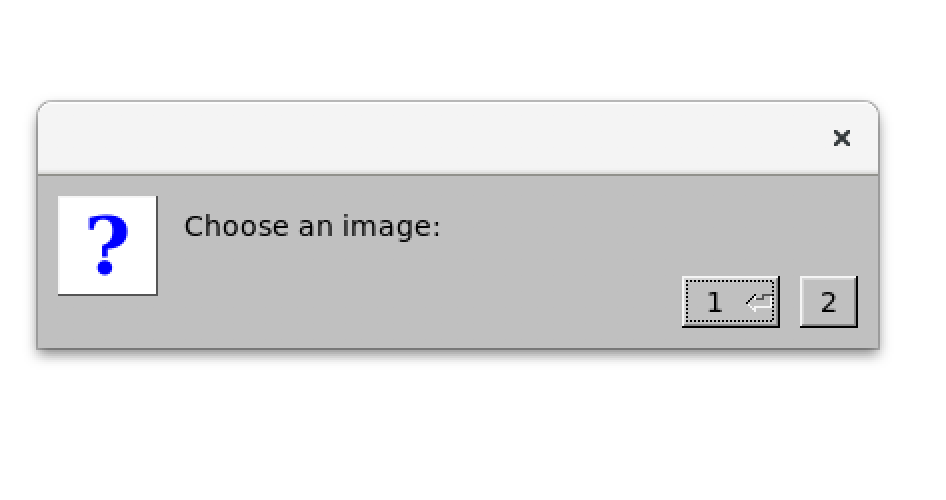
\includegraphics[width = 10cm, height = 5cm]{ci.png}
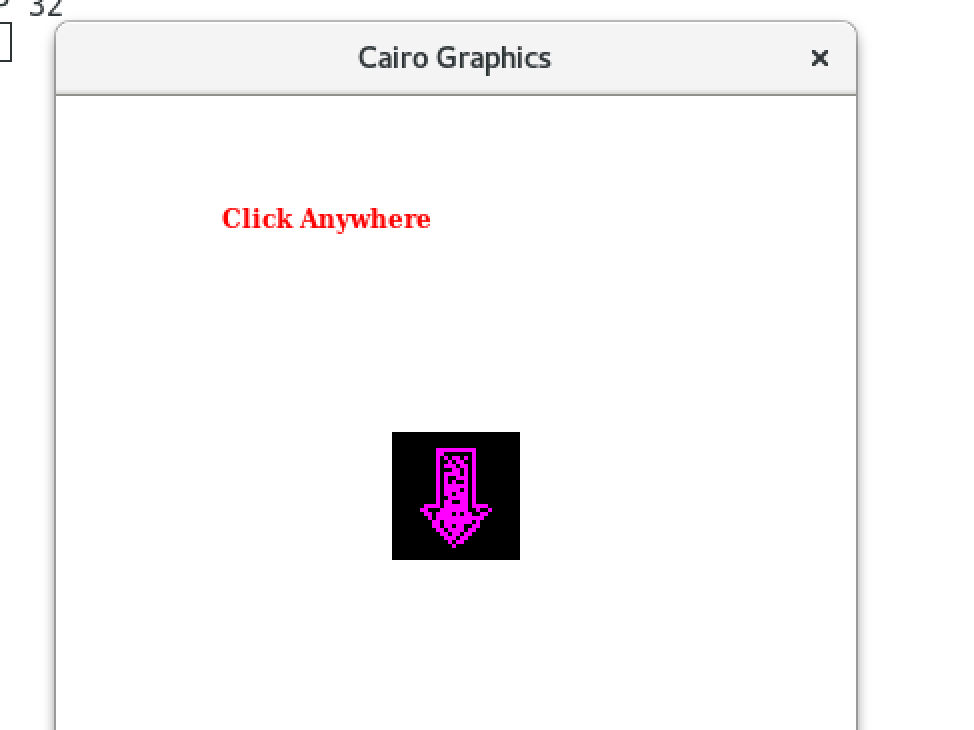
\includegraphics[width = 10cm, height = 6cm]{ci1.png}
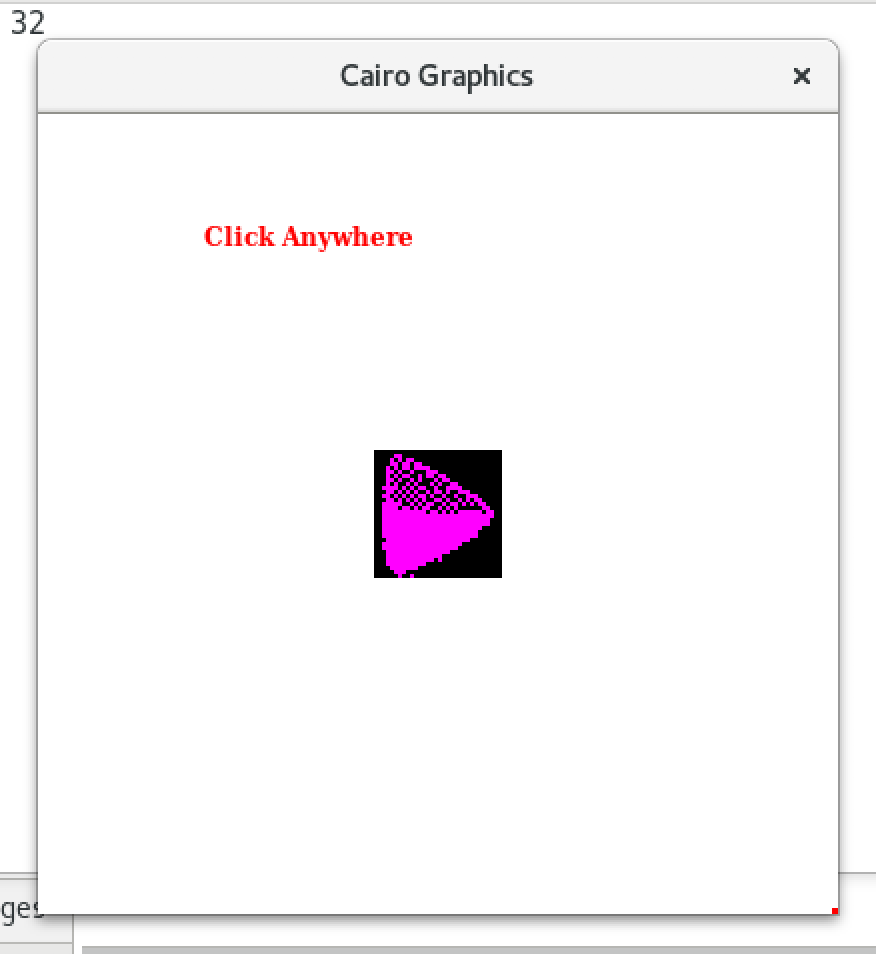
\includegraphics[width = 9cm, height = 7cm]{ci2.png}
\newpage

\subsection*{Testcase of resize by 2 or 3(it runs well)}
\begin{itemize}
	\item When the user execute our program,select an image,the user can click either of these two resize buttons to resize the image by 2 or 3.
\end{itemize}
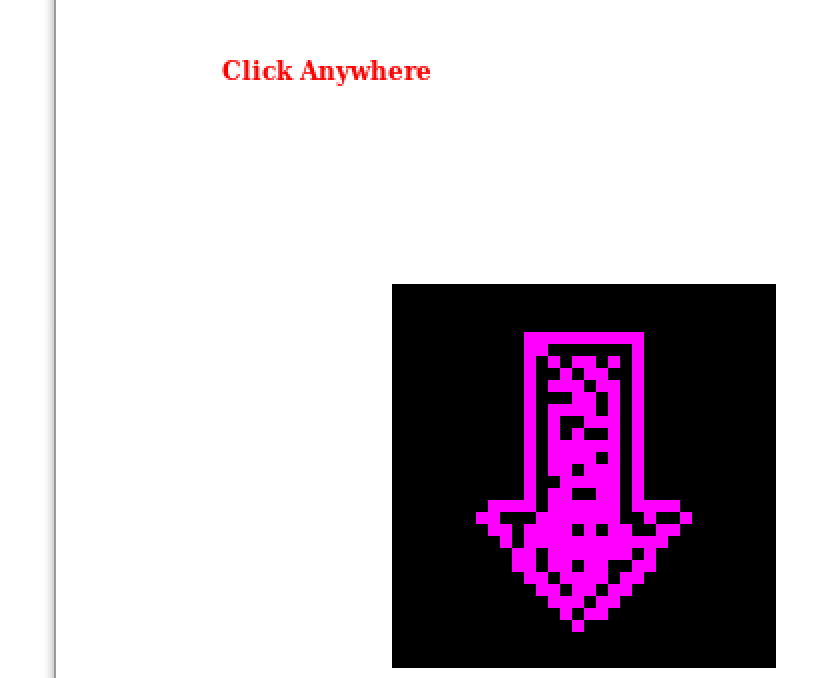
\includegraphics[width = 10cm, height = 8cm]{r3.png}
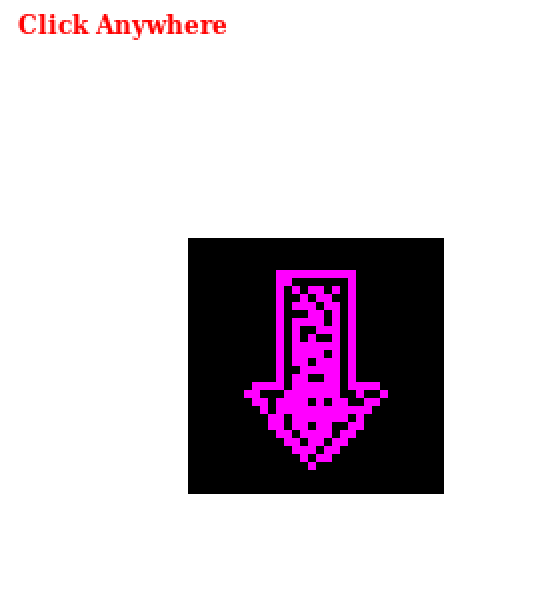
\includegraphics[width = 7cm, height = 8cm]{r2.png}
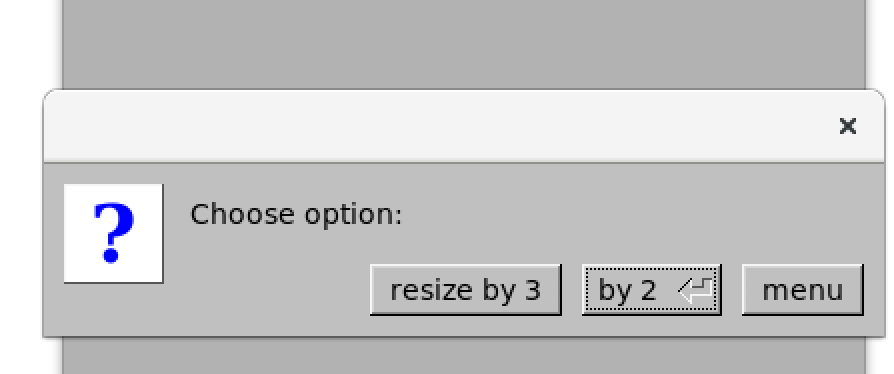
\includegraphics[width = 8cm, height = 3cm]{5.png}
\newpage

\subsection*{Testcase of enter the menu(it runs well)}
\begin{itemize}
	\item When the user execute our program,select an image,the user can click the menu button to enter the menu,where the user can modify the image.
\end{itemize}
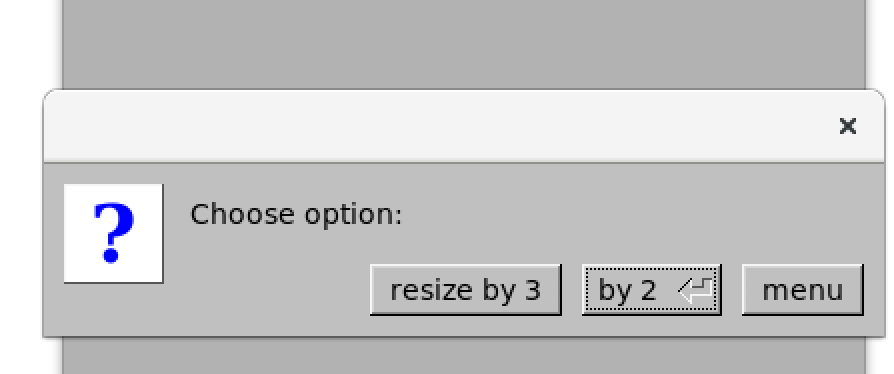
\includegraphics[width = 8cm, height = 4cm]{5.png}
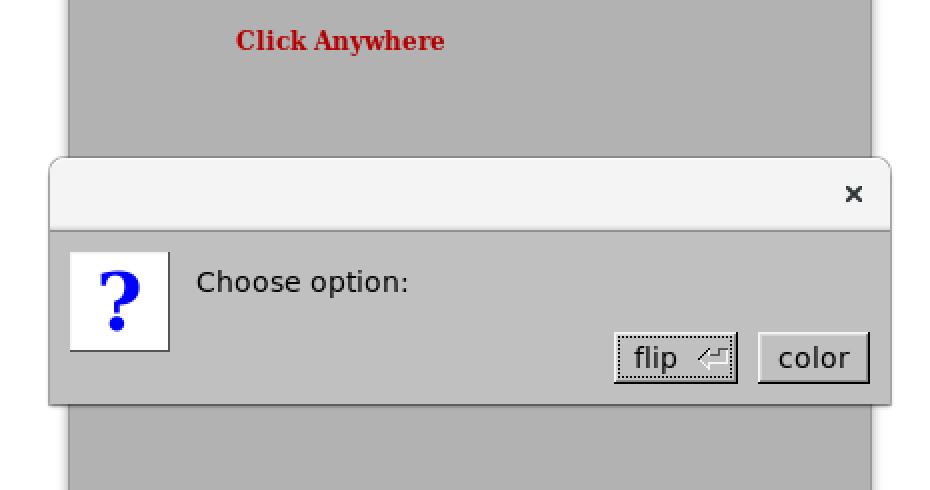
\includegraphics[width = 8cm, height = 4cm]{4.png}
\newpage

\subsection*{Testcase of flip vertically(it runs well)}
\begin{itemize}
	\item When the user execute our program,select an image,enter the menu,the user can click one of the three buttons to modify the image.If the user choose flip and then choose vertical,the image will be flipped vertically.
\end{itemize}
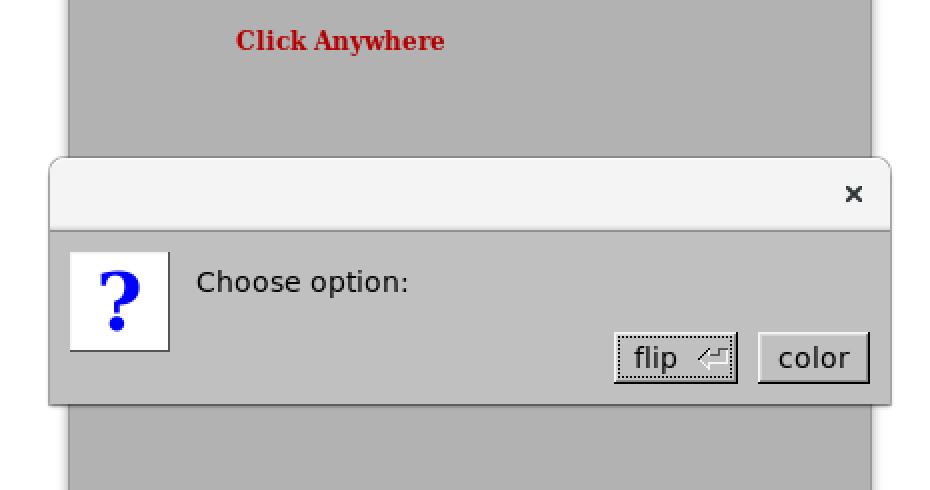
\includegraphics[width = 8cm, height = 4cm]{4.png}
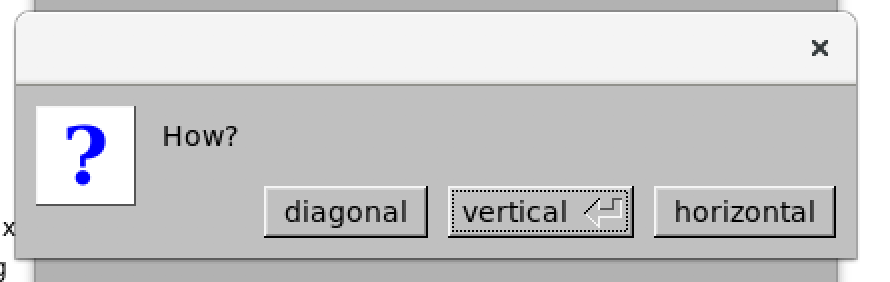
\includegraphics[width = 10cm, height = 4cm]{v1.png}
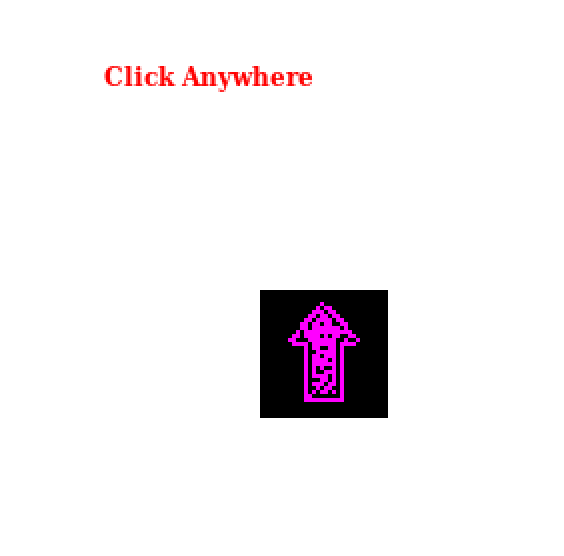
\includegraphics[width = 10cm, height = 7cm]{v2.png}
\newpage

\subsection*{Testcase of flip horizontally (it runs well)}
\begin{itemize}
	\item When the user execute our program,select an image,enter the menu,the user can click one of the three buttons to modify the image(flip or change color).If the user choose flip and then choose horizontal,the image will be flipped horizontally.
\end{itemize}
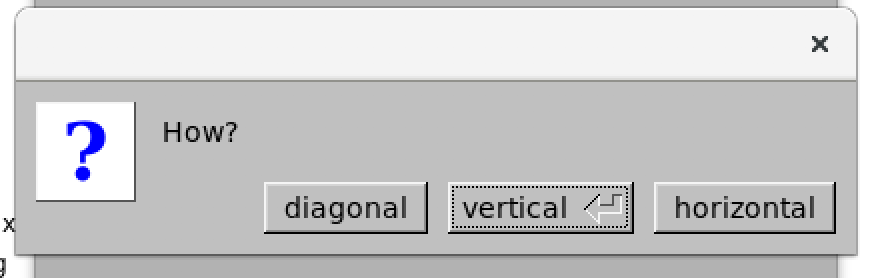
\includegraphics[width = 10cm, height = 4cm]{h1.png}
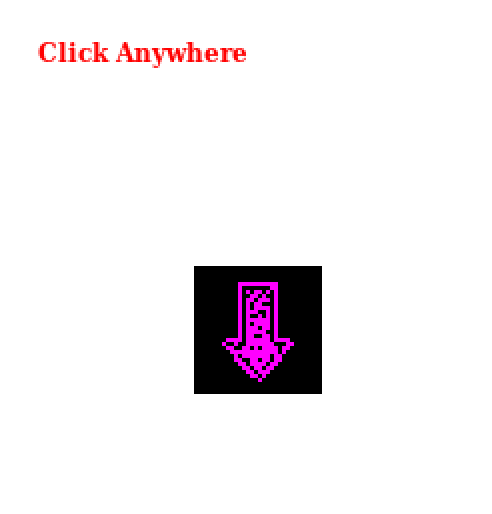
\includegraphics[width = 10cm, height = 8cm]{h2.png}

\subsection*{Testcase of mirror image across diagonal(it runs well)}
\begin{itemize}
	\item When the user execute our program,select an image,enter the menu,the user can click one of the three buttons to modify the image(flip or change color).If the user choose flip and then choose diagonal, and one of the two diagonals, the image will be flipped horizontally by that diagonal.
\end{itemize}
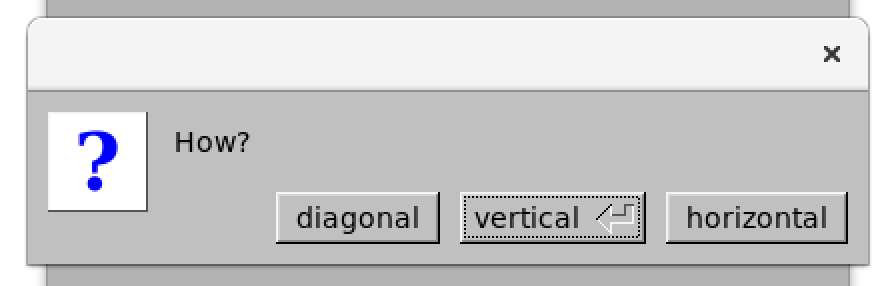
\includegraphics[width = 10cm, height = 4cm]{d.png}
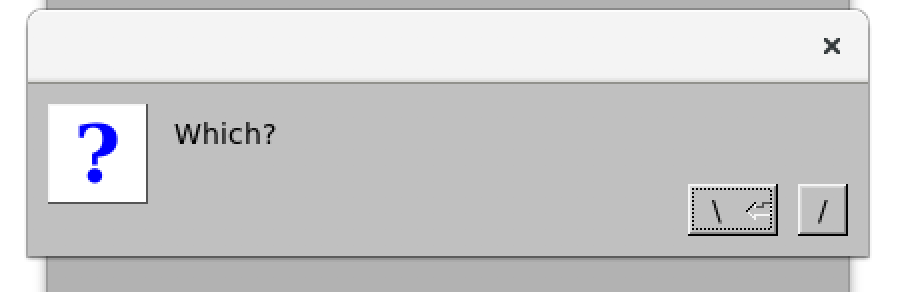
\includegraphics[width = 8cm, height = 3cm]{d2.png}
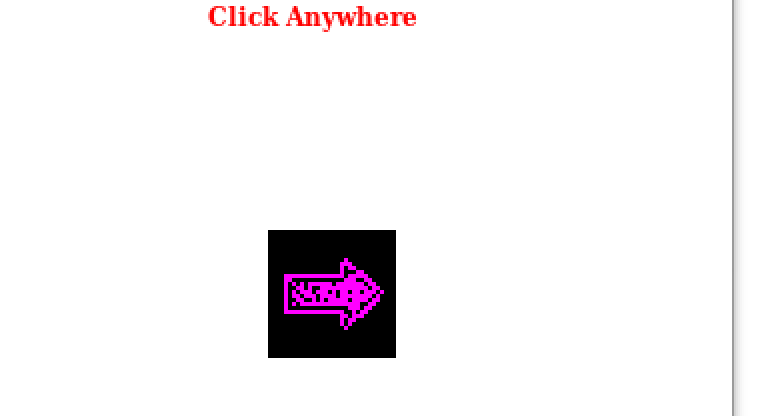
\includegraphics[width = 13cm, height = 7cm]{d3.png}

\includegraphics[width = 8cm, height = 7cm]{d4.png}
\newpage

\subsection*{Testcase of invert the 2 colors(it runs well)}
\begin{itemize}
	\item When the user execute our program,select an image,enter the menu,the user can click one of the three buttons to modify the image(flip or change color).If the user choose color and then choose inverse,the 2 colors will be inverted.
\end{itemize}
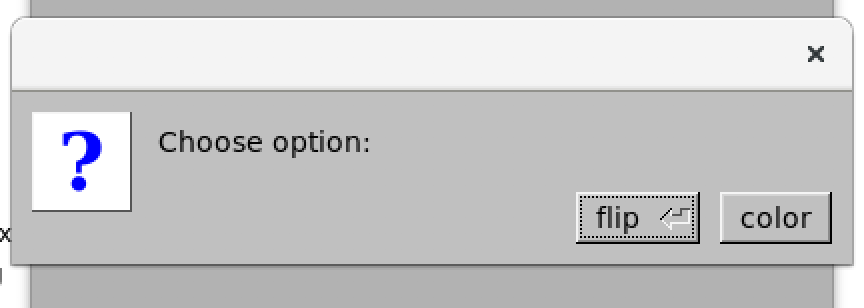
\includegraphics[width = 10cm, height = 4cm]{i1.png}
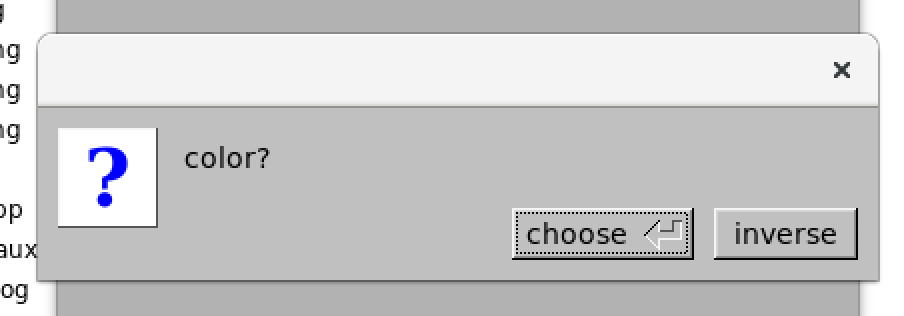
\includegraphics[width = 8cm, height = 4cm]{i2.png}
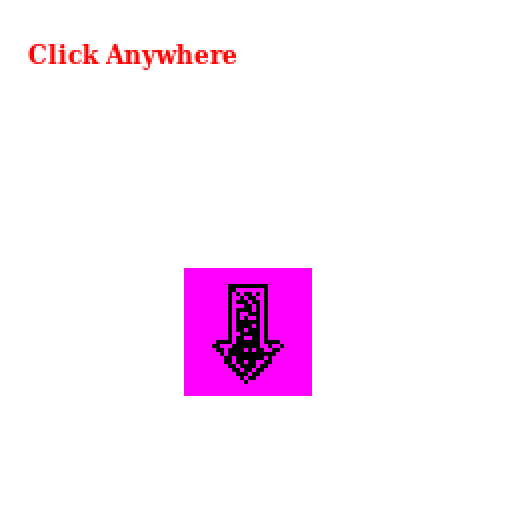
\includegraphics[width = 9cm, height = 7cm]{i3.png}

\subsection*{Testcase of choose colors(it runs well)}
\begin{itemize}
	\item When the user execute our program,select an image,enter the menu,the user can click one of the three buttons to modify the image(flip or change color).If the user choose color and then choose choose,the user can choose the color of the image.
\end{itemize}
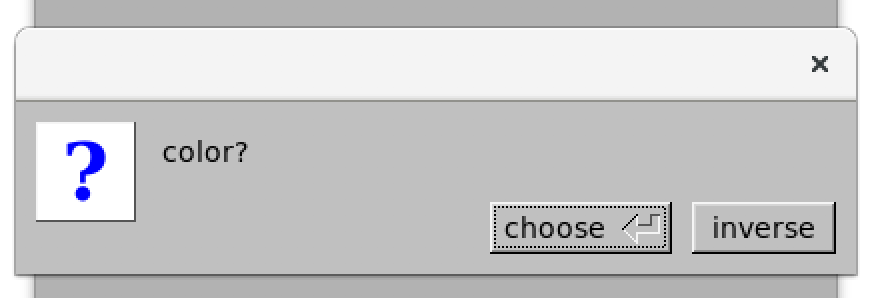
\includegraphics[width = 10cm, height = 4cm]{cc1.png}
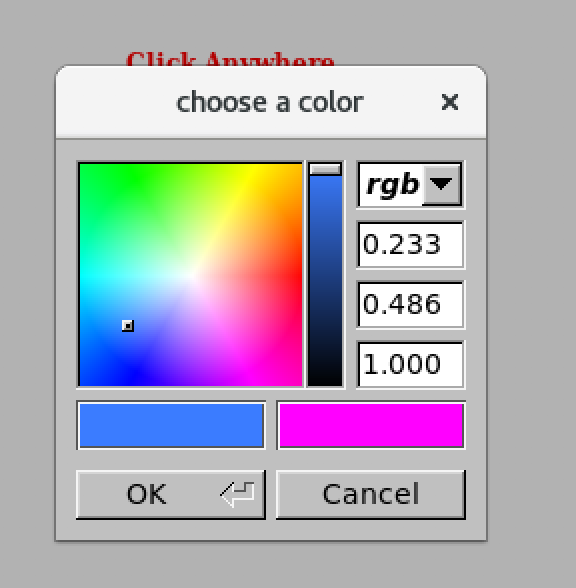
\includegraphics[width = 8cm, height = 7cm]{cc2.png}
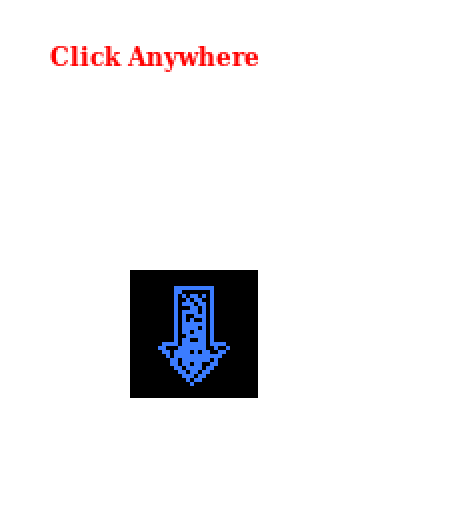
\includegraphics[width = 9cm, height = 8cm]{cc3.png}

\subsection*{Conclusion of my testcases}
	
\includegraphics[width = 10cm, height = 9cm]{happy.png}
\begin{description}
	\item As we can see in my testcases, all of my codes run well.
	\item I successfully acheived the goal of this lab assignment!
\end{description}
\end{document}
